\section*{Experiment 3}

In this experiment, we constructed a two-way current divider, with the divider ratio is a ratio of
two small integers by connecting them in series and in parallel. We used two \nMOS transistors in series for one branch of the current dividers, and two \nMOS transistors in parallel for the other current. We took turns setting the input of the current divider at the sources of both branches and then the drain of both branches, as shown in figures \ref{fig:exp3p1dia} and \ref{fig:exp3p2dia}.

From the pre-lab, we know that two transistors in series with unit strength ratios act as a single \nMOS transistor with strength ratio $\frac{1}{2}$, and that two \nMOS transistors in parallel act as a single \nMOS transistor with strength ratio 2. We attached the SMU probe to the drains of the two parallel \nMOS transistors while tying the drain of the series \nMOS branch to \Vdd. In the prelab we also showed that for an \nMOS current divider, the ratio between the current of a branch $I_1$ to the total current $I$ is $$\frac{I_2}{I} = \frac{S_2}{S_2S_1}$$, where $S_1$ and $S_2$ are the equivalent strength ratios of each branch. Therefore, for both current dividers we tested, we expected the current divider ratio to be $$\frac{I_{out}}{I_{in}} = \frac{2}{2 + \frac{1}{2}} = \frac{4}{5}$$


\begin{figure}[H]
\centering
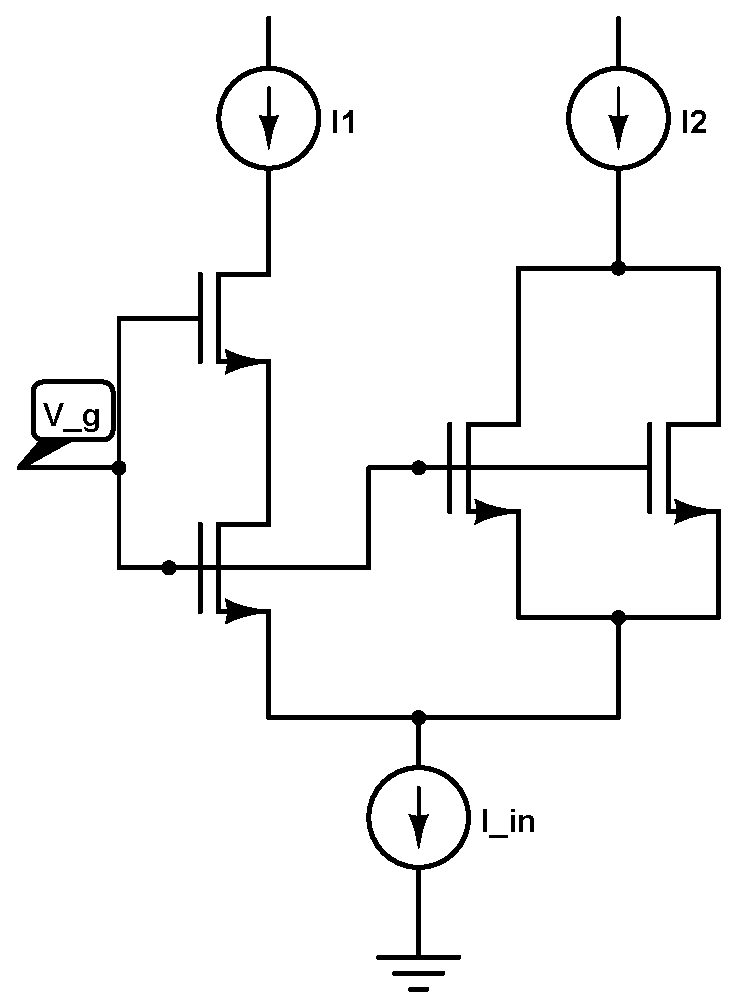
\includegraphics[width=0.65\linewidth]{../Figures/Experiment3CircuitDiagram1.eps}
\caption{A diagram of the circuit used in Experiment 3.}
\label{fig:exp3p1dia}
\end{figure}

We first set \Iin using the sources of both branches of the current divider, and measured \Iout as a function of \Iin as we varied \Iin on a log scale. We attached the SMU leads to the parallel transistor branch, so we expected a current divider ratio of 0.8. As figure \ref{fig:exp3p1} shows, the current transistor characteristic of the circuit is very linear on a log scale, and we confirmed using \texttt{polyfit} that the slope of the line was 0.7870, which is very close to the predicted ratio of 0.8.

We can see that the theoretical fit, which was created by multiplying \Iin 0.8, matches the data very closely through many orders of magnitude of \Iin. This indicates that this current divider can be expected to operate as theoretically predicted for many values of \Iin.

\begin{figure}[H]
\centering
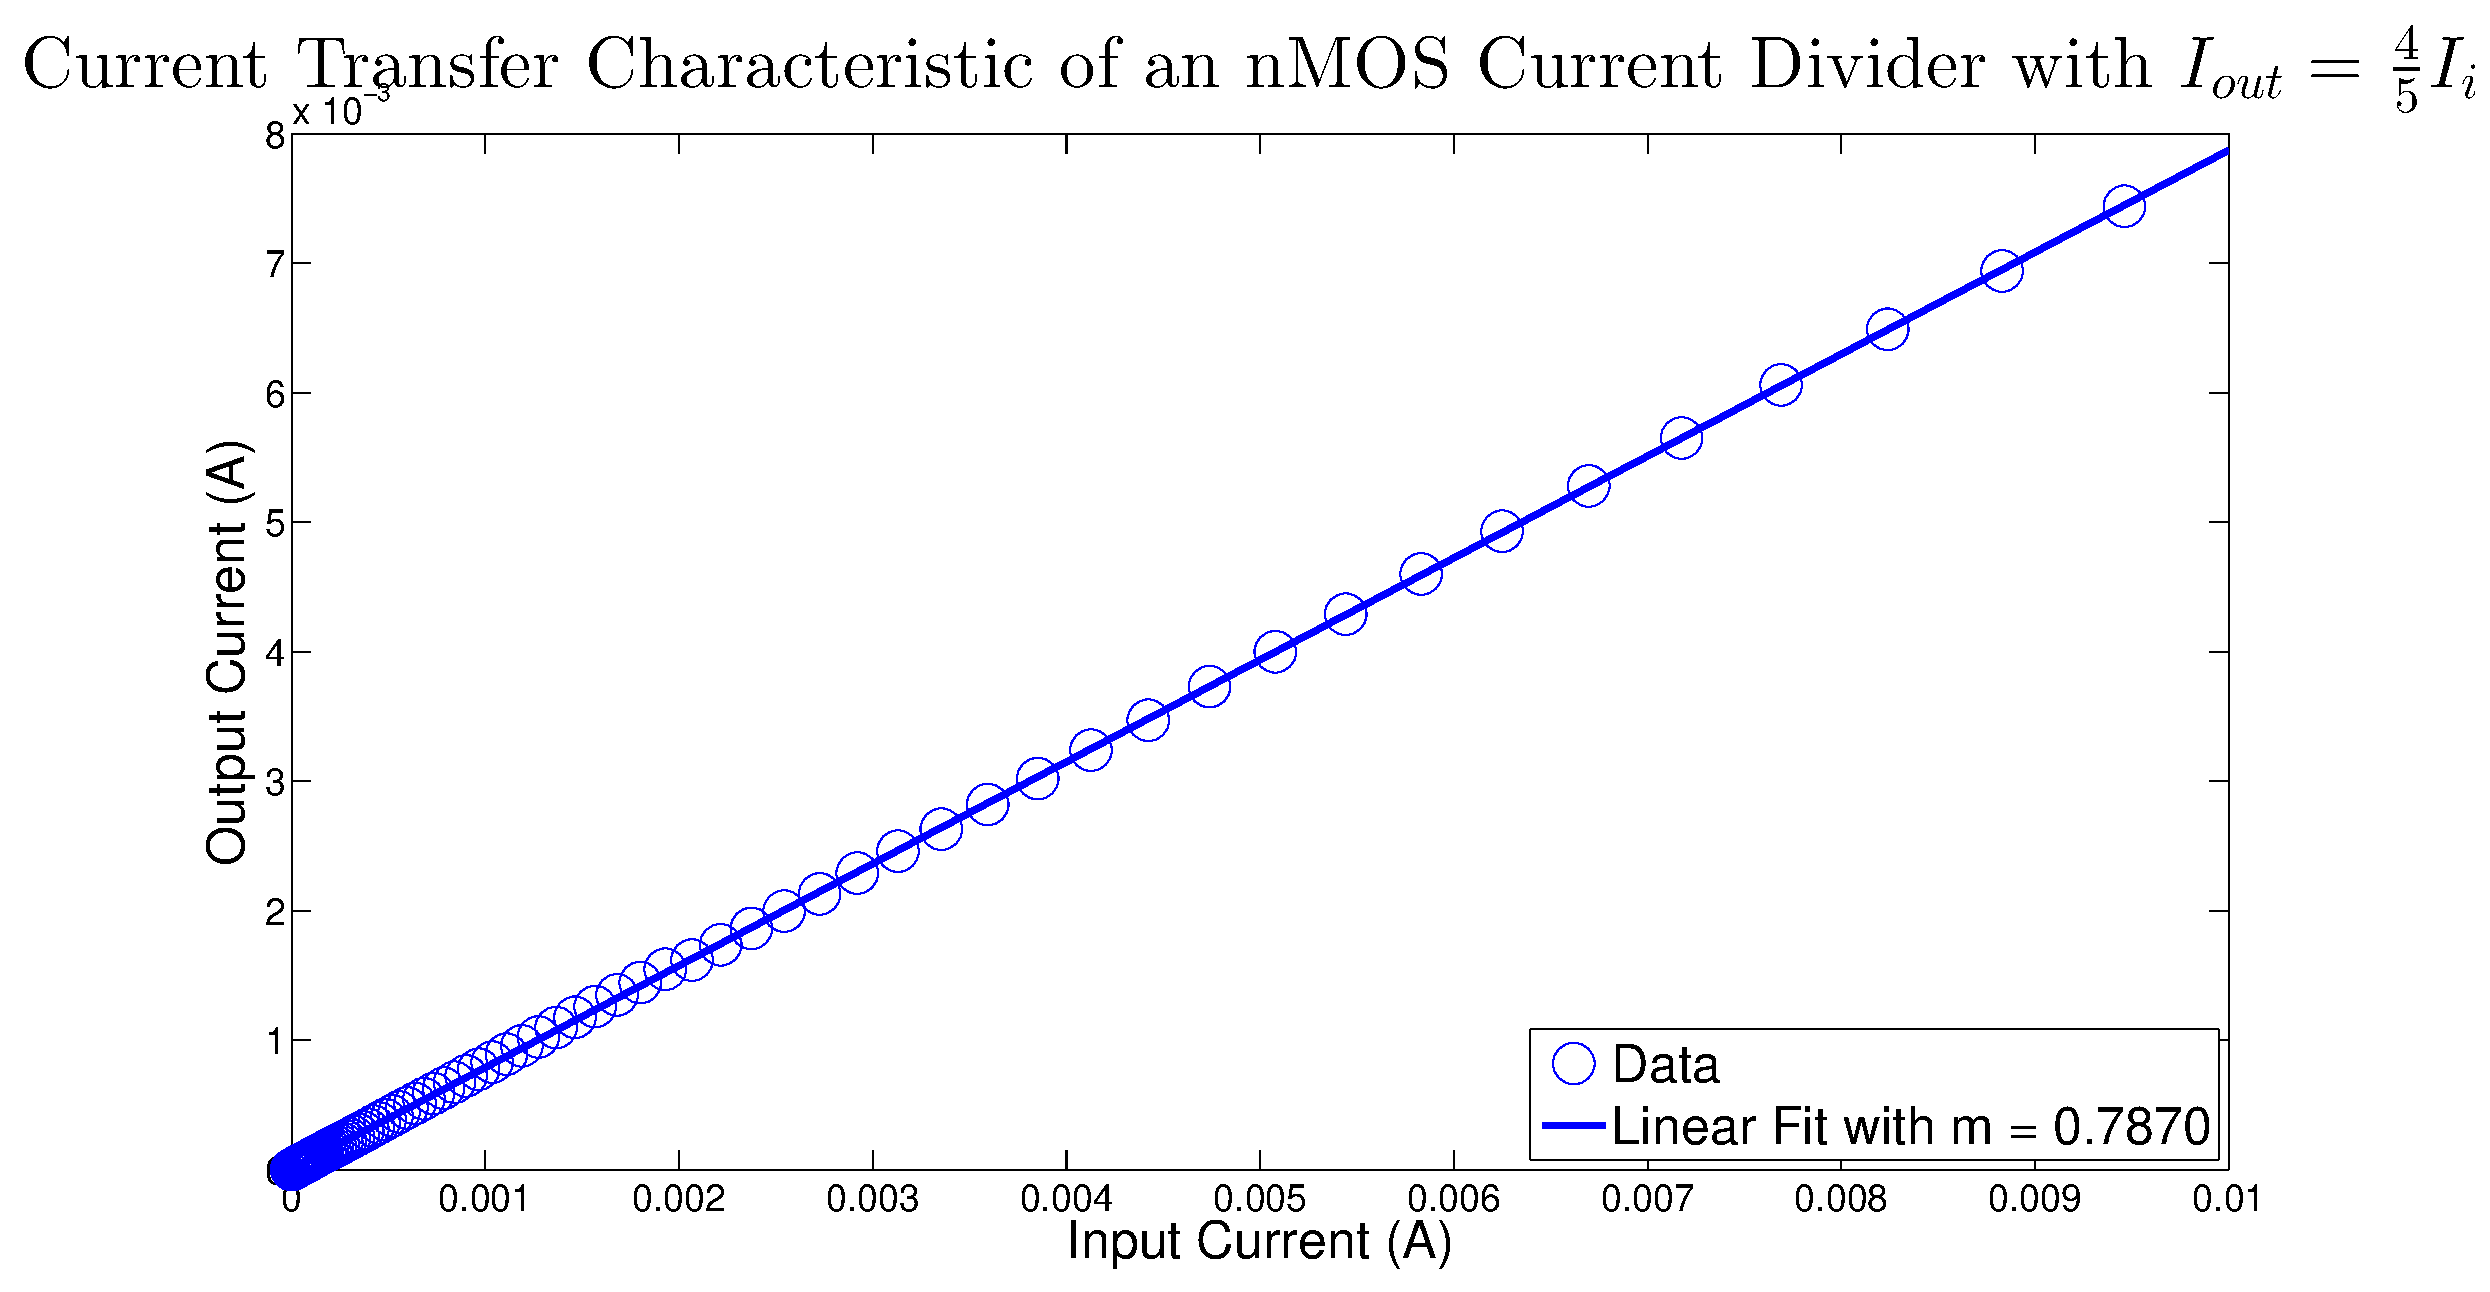
\includegraphics[width=\linewidth]{../Figures/Experiment3Figure1.eps}
\caption{A diagram of the circuit used in Experiment 3.}
\label{fig:exp3p2}
\end{figure}

\begin{figure}[H]
\centering
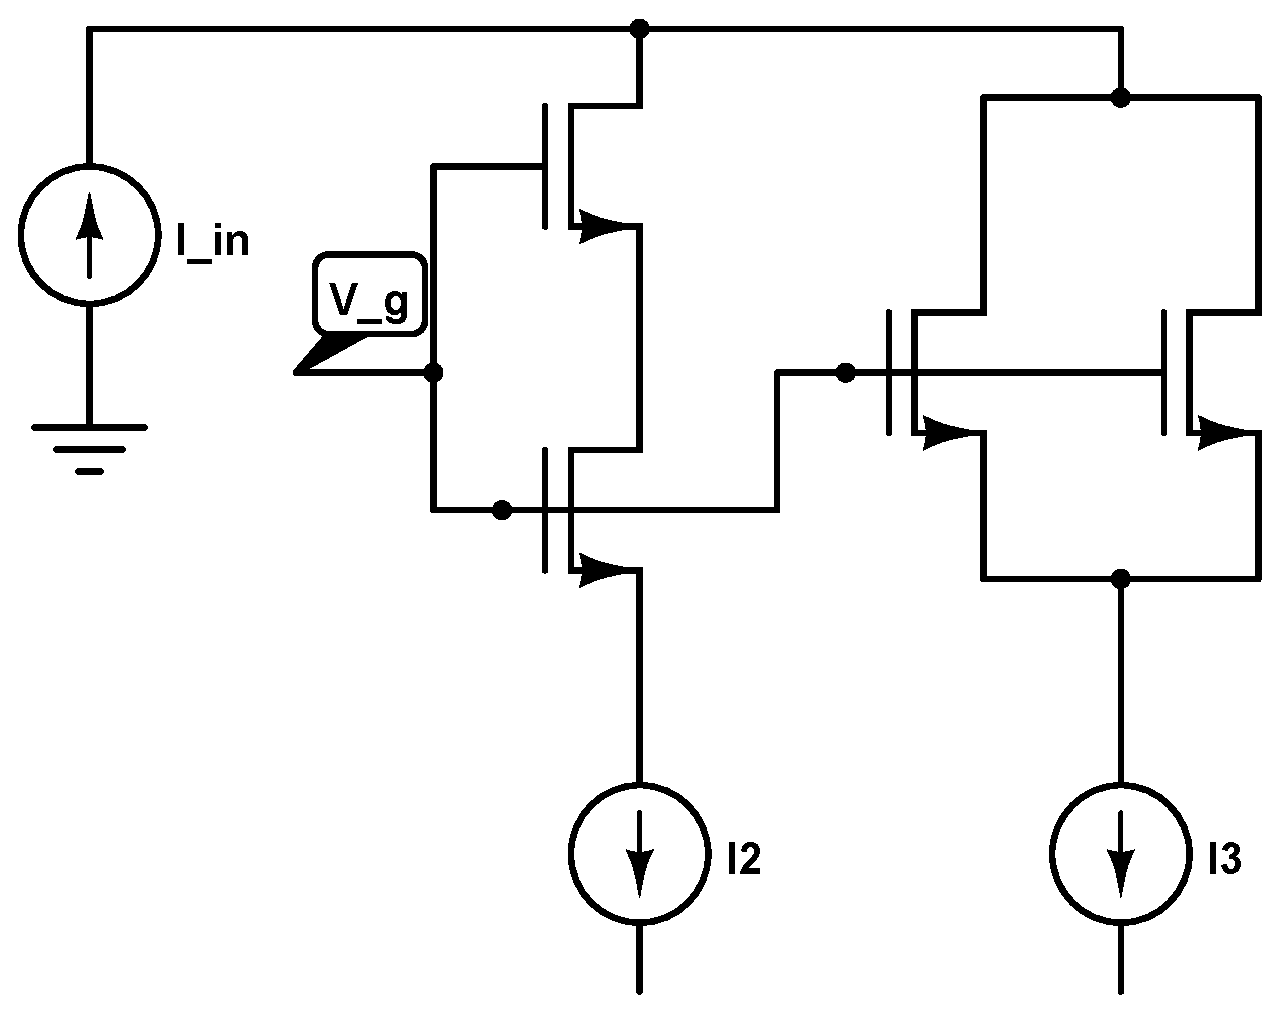
\includegraphics[width=0.65\linewidth]{../Figures/Experiment3CircuitDiagram2.eps}
\caption{A diagram of the circuit used in Experiment 3.}
\label{fig:exp3p2dia}
\end{figure}


\begin{figure}[H]
\centering
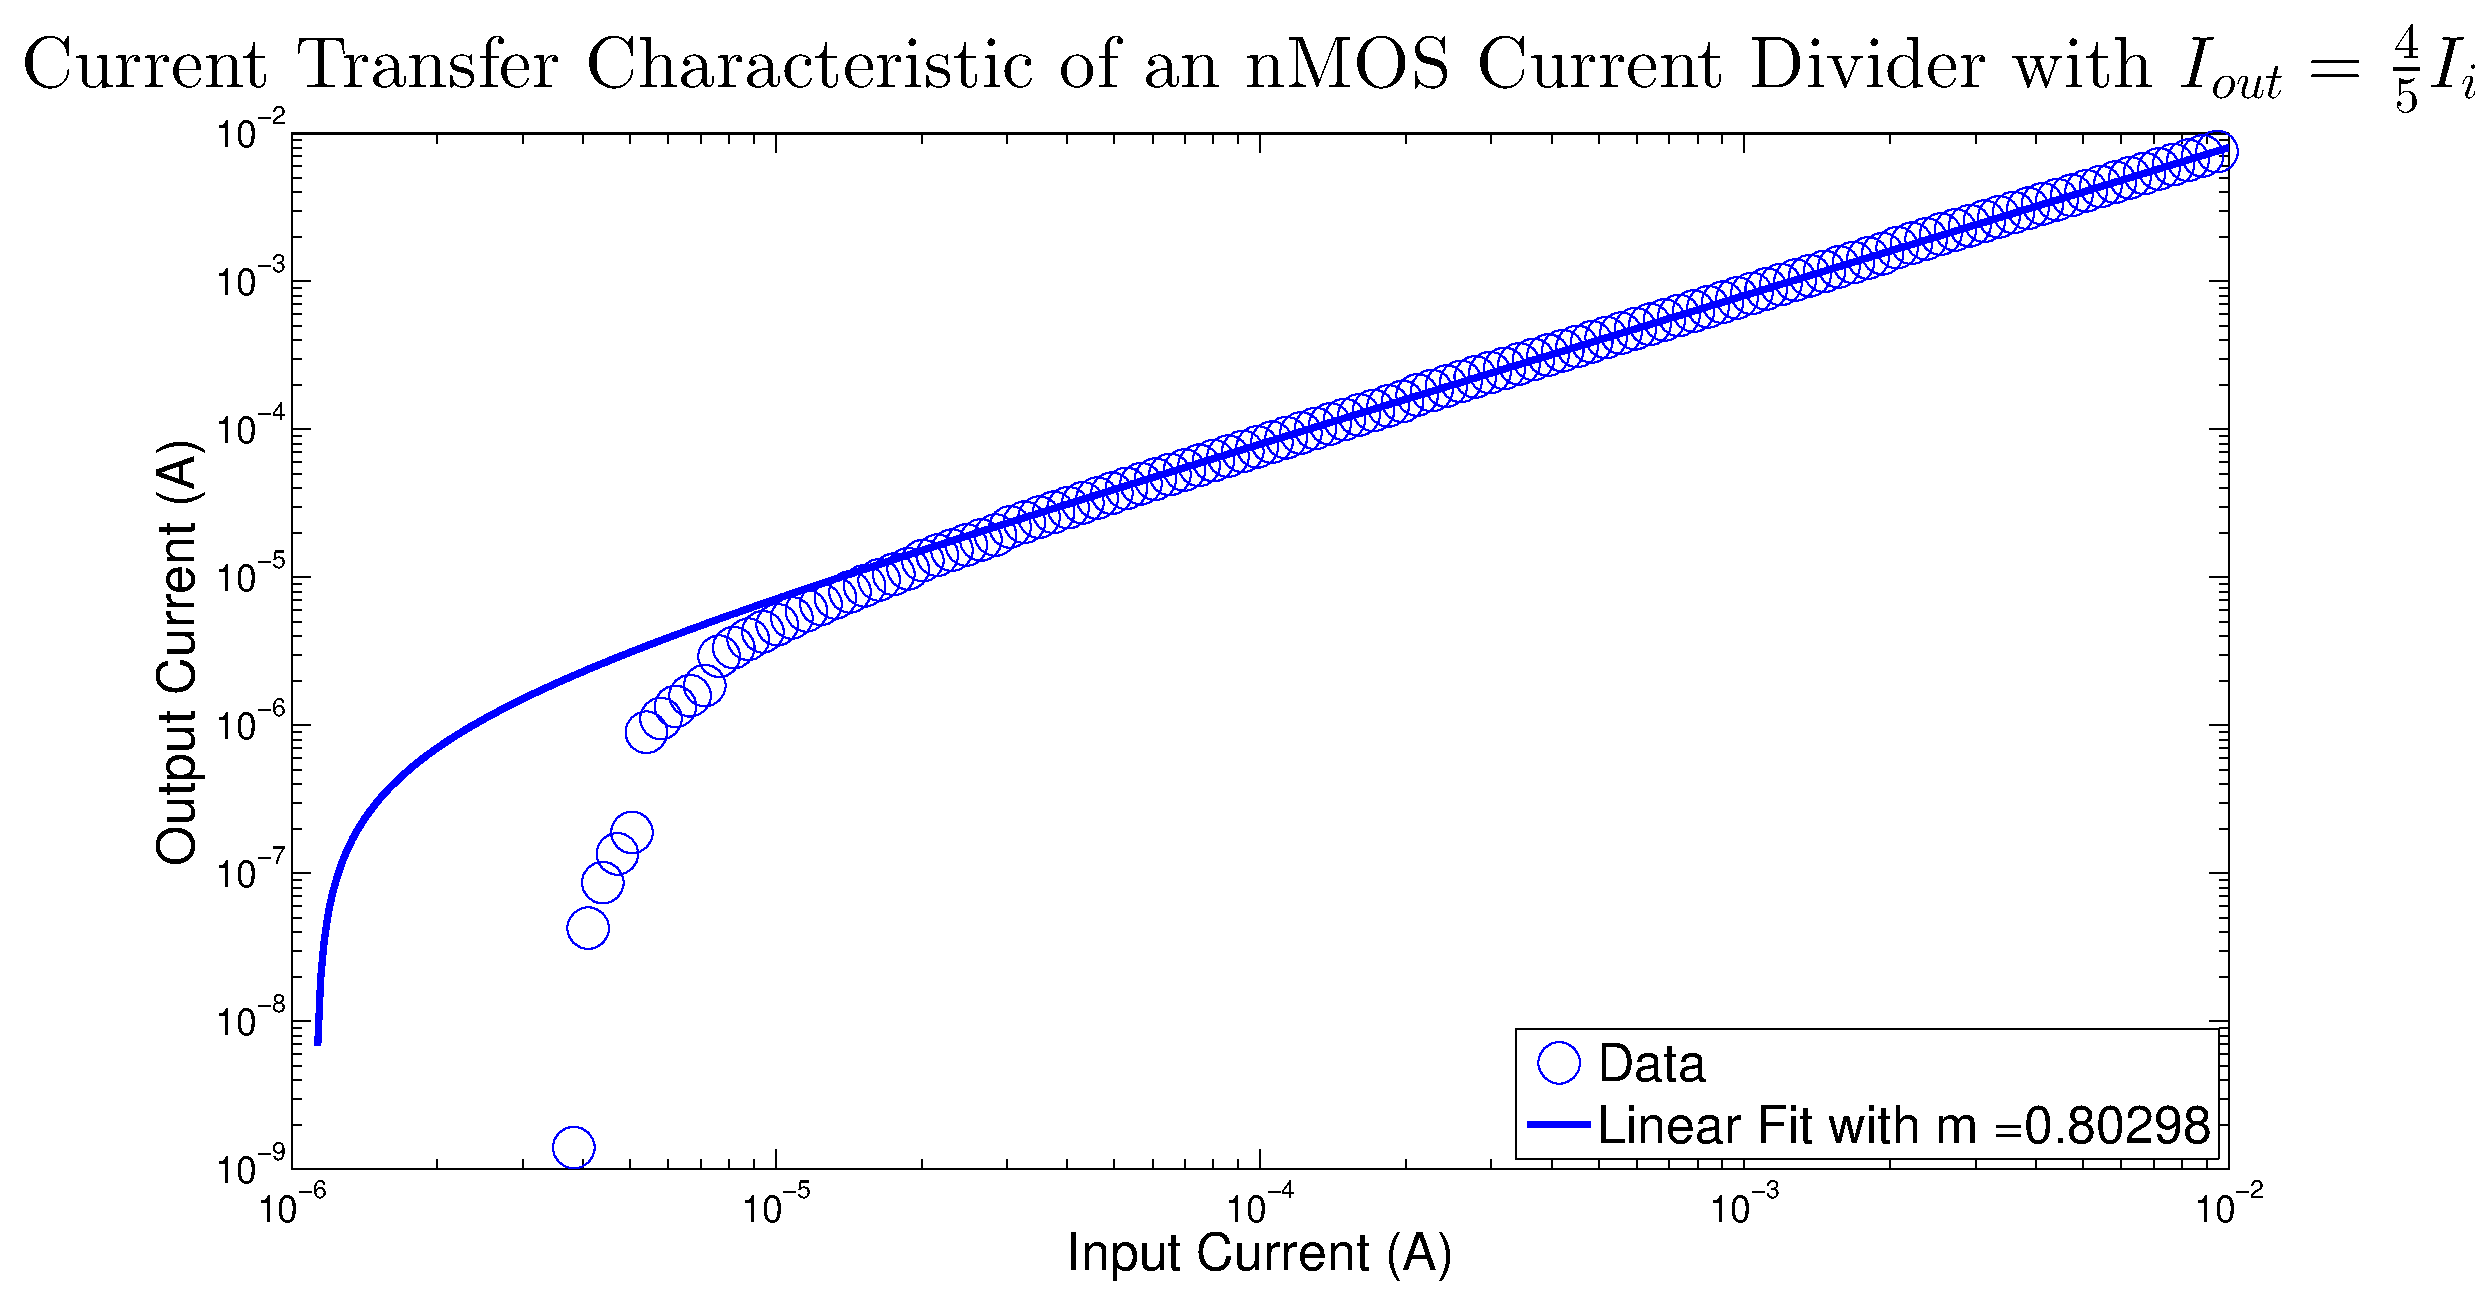
\includegraphics[width=\linewidth]{../Figures/Experiment3Figure2.eps}
\caption{A diagram of the circuit used in Experiment 3.}
\label{fig:exp3p2}
\end{figure}